% This is "sig-alternate.tex" V2.0 May 2012
% This file should be compiled with V2.5 of "sig-alternate.cls" May 2012
%
% This example file demonstrates the use of the 'sig-alternate.cls'
% V2.5 LaTeX2e document class file. It is for those submitting
% articles to ACM Conference Proceedings WHO DO NOT WISH TO
% STRICTLY ADHERE TO THE SIGS (PUBS-BOARD-ENDORSED) STYLE.
% The 'sig-alternate.cls' file will produce a similar-looking,
% albeit, 'tighter' paper resulting in, invariably, fewer pages.
%
% ----------------------------------------------------------------------------------------------------------------
% This .tex file (and associated .cls V2.5) produces:
%       1) The Permission Statement
%       2) The Conference (location) Info information
%       3) The Copyright Line with ACM data
%       4) NO page numbers
%
% as against the acm_proc_article-sp.cls file which
% DOES NOT produce 1) thru' 3) above.
%
% Using 'sig-alternate.cls' you have control, however, from within
% the source .tex file, over both the CopyrightYear
% (defaulted to 200X) and the ACM Copyright Data
% (defaulted to X-XXXXX-XX-X/XX/XX).
% e.g.
% \CopyrightYear{2007} will cause 2007 to appear in the copyright line.
% \crdata{0-12345-67-8/90/12} will cause 0-12345-67-8/90/12 to appear in the copyright line.
%
% ---------------------------------------------------------------------------------------------------------------
% This .tex source is an example which *does* use
% the .bib file (from which the .bbl file % is produced).
% REMEMBER HOWEVER: After having produced the .bbl file,
% and prior to final submission, you *NEED* to 'insert'
% your .bbl file into your source .tex file so as to provide
% ONE 'self-contained' source file.
%
% ================= IF YOU HAVE QUESTIONS =======================
% Questions regarding the SIGS styles, SIGS policies and
% procedures, Conferences etc. should be sent to
% Adrienne Griscti (griscti@acm.org)
%
% Technical questions _only_ to
% Gerald Murray (murray@hq.acm.org)
% ===============================================================
%
% For tracking purposes - this is V2.0 - May 2012

%\documentclass[10pt, conference, compsocconf]{IEEEtran}
\documentclass[10pt,conference]{IEEEtran}
%\documentclass{sig-alternate}
\usepackage{url}
\usepackage{balance}
\usepackage{hyperref}
\usepackage{graphicx}
\usepackage{xspace}
\usepackage{color}
\usepackage{pifont}
\sloppy

\newcommand {\pat}[1]{[{\bf \underline{Patrizio}}: {\bf #1}]}
\newcommand{\todo}[1]{\textcolor{blue}{\ding{46}~{\sf todo}~#1}}

%\newcommand{\definition}[2]{\noindent \textbf{\emph{Definition #1}} (#2)}
\newcommand{\ttransition}[2]{\stackrel{#1}{\longrightarrow^{#2}}}
\newcommand{\ntransition}[1]{\longrightarrow^{#1}}
\newcommand{\transition}[1]{\stackrel{#1}{\rightarrow}}
\newcommand{\Transition}[1]{\stackrel{#1}{\Rightarrow}}
\newcommand{\freccia}[1]{\mathop{\stackrel{#1} {\longrightarrow}} }
\newcommand{\ug}[1]{\mathop{=}\limits^{#1}_{}}
\newcommand{\barra}[1]{\overline{#1}}
\newcommand{\eqdef}{\stackrel{def}{=}}


\newcommand{\footlabel}[2]{%
    \addtocounter{footnote}{1}%
    \footnotetext[\thefootnote]{%
        \addtocounter{footnote}{-1}%
        \refstepcounter{footnote}\label{#1}%
        {\footnotesize #2}%
    }%
    $^{\ref{#1}}$%
}

\newcommand{\footref}[1]{%
    $^{\ref{#1}}$%
}

\newcommand{\approach}{Postmonkey}


\usepackage{listings}

% colors
\definecolor{mygreen}{rgb}{0,0.6,0}
\definecolor{mygray}{rgb}{0.5,0.5,0.5}
\definecolor{mymauve}{rgb}{0.58,0,0.82}
\definecolor{light-gray}{gray}{0.85}

% listing settings
\lstset{ %
  backgroundcolor=\color{white},   % choose the background color; you must add \usepackage{color} or \usepackage{xcolor}
  basicstyle=\footnotesize,        % the size of the fonts that are used for the code
  breakatwhitespace=false,         % sets if automatic breaks should only happen at whitespace
  breaklines=true,                 % sets automatic line breaking
  captionpos=b,                    % sets the caption-position to bottom
  commentstyle=\color{mygreen},    % comment style
  deletekeywords={...},            % if you want to delete keywords from the given language
  escapeinside={\%*}{*)},          % if you want to add LaTeX within your code
  extendedchars=true,              % lets you use non-ASCII characters; for 8-bits encodings only, does not work with UTF-8
  frame=single,                    % adds a frame around the code
  keepspaces=true,                 % keeps spaces in text, useful for keeping indentation of code (possibly needs columns=flexible)
  keywordstyle=\color{blue},       % keyword style
  language=C,                      % the language of the code
  morekeywords={*,...},            % if you want to add more keywords to the set
  numbers=left,                    % where to put the line-numbers; possible values are (none, left, right)
  numbersep=5pt,                   % how far the line-numbers are from the code
  numberstyle=\tiny\color{mygray}, % the style that is used for the line-numbers
  rulecolor=\color{black},         % if not set, the frame-color may be changed on line-breaks within not-black text (e.g. comments (green here))
  showspaces=false,                % show spaces everywhere adding particular underscores; it overrides 'showstringspaces'
  showstringspaces=false,          % underline spaces within strings only
  showtabs=false,                  % show tabs within strings adding particular underscores
  stepnumber=1,                    % the step between two line-numbers. If it's 1, each line will be numbered
  stringstyle=\color{mymauve},     % string literal style
  tabsize=2,                       % sets default tabsize to 2 spaces
  caption=A program                % show the filename of files included with \lstinputlisting; also try caption instead of title
}


\begin{document}


\title{Towards Online Testing of Distributed Embedded Systems: an Industrial Experience}

%\title{Testing of Distributed Embedded Systems: an Industrial Experience}



\author{\IEEEauthorblockN{Zhenxiao Hao\IEEEauthorrefmark{1}, Khaled Alnawasreh\IEEEauthorrefmark{1}, Patrizio Pelliccione\IEEEauthorrefmark{1},  M\aa rten R\aa nge\IEEEauthorrefmark{2}, and Antonia Bertolino\IEEEauthorrefmark{3}}
\IEEEauthorblockA{\IEEEauthorrefmark{1}Chalmers University of Technology $|$ University of Gothenburg\\
Department of Computer Science and Engineering,
Gothenburg, Sweden\\
Email: zhenxiao@student.chalmers.se, khaled.nawasreh@gmail.com, patrizio.pelliccione@gu.se}
%\and
\IEEEauthorblockA{\IEEEauthorrefmark{2}Ericsson AB, Gothenburg, Sweden}
\IEEEauthorblockA{\IEEEauthorrefmark{3}ISTI - CNR, Via G. Moruzzi 1, 56124 Pisa, Italy}
%\IEEEauthorblockA{
%Email: name@xyz.com}
}

% conference papers do not typically use \thanks and this command
% is locked out in conference mode. If really needed, such as for
% the acknowledgment of grants, issue a \IEEEoverridecommandlockouts
% after \documentclass

% for over three affiliations, or if they all won't fit within the width
% of the page, use this alternative format:
% 
%\author{\IEEEauthorblockN{Michael Shell\IEEEauthorrefmark{1},
%Homer Simpson\IEEEauthorrefmark{2},
%James Kirk\IEEEauthorrefmark{3}, 
%Montgomery Scott\IEEEauthorrefmark{3} and
%Eldon Tyrell\IEEEauthorrefmark{4}}
%\IEEEauthorblockA{\IEEEauthorrefmark{1}School of Electrical and Computer Engineering\\
%Georgia Institute of Technology,
%Atlanta, Georgia 30332--0250\\ Email: see http://www.michaelshell.org/contact.html}
%\IEEEauthorblockA{\IEEEauthorrefmark{2}Twentieth Century Fox, Springfield, USA\\
%Email: homer@thesimpsons.com}
%\IEEEauthorblockA{\IEEEauthorrefmark{3}Starfleet Academy, San Francisco, California 96678-2391\\
%Telephone: (800) 555--1212, Fax: (888) 555--1212}
%\IEEEauthorblockA{\IEEEauthorrefmark{4}Tyrell Inc., 123 Replicant Street, Los Angeles, California 90210--4321}}





\maketitle
\begin{abstract}
Having robust systems that are able to perform normally even with the existence of faults is becoming increasingly important. This is the case of the embedded distributed system in the RBS (Radio Based Station) at Ericsson AB in Gothenburg, Sweden, which we investigate in this paper. Specifically, this paper describes a novel fault injection approach for %online 
testing the robustness of an embedded distributed system consisting of components that communicate with each other via messages exchange. 
The new approach is inspired by Netflix's ChaosMonkey, a fault injection approach that has been developed for testing the distributed systems hosted on the cloud. In the context of RBS we cannot use ChaosMonkey as it is since 
RBS is a distributed system consisting of small-embedded components with specific requirements of performance, programming language, and communication paradigm.
This paper reports about the approach we developed, called \approach{}\footnote{\approach{} is a portmanteau fusing the word Postman and Monkey. The rational is that the approach is inspired by ChaosMonkey and applies it at the level of message exchange (content and delay) - this is why Postman.},  the faults we discovered though the use of the approach, and discusses about the potential of utilizing fault injection to %online 
testing complex, embedded, and distributed systems. The approach and tool are now adopted by Ericsson.
\end{abstract}

\begin{IEEEkeywords}
online testing; fault injection; distributed embedded systems;

\end{IEEEkeywords}

\IEEEpeerreviewmaketitle

\section{Introduction}
    
%%Due to the evolution of social media and mobile devices, massive network data is produced. 
%Distributed systems are at the core of the evolution of social media and mobile devices. This evolution leads to the creation of massive network data and efficient manipulation and usage of network data is becoming a major issue.  In order to process network data in parallel and perform tasks efficiently, many computing nodes are connected, providing users with services characterized by fault tolerance, ease of use and speed~\cite{tanenbaum}.
 
%Services running in distributed systems are difficult to be tested using traditional methods \cite{FaaS}. When faults occur in running services, faults can exponentially propagate \cite{verification_testing}. In this case, identifying faults in a running application in a production environment would go a long way. Testing in large scale distributed system is very hard due to the fact that the number of faults that can occur at any time is very large as well as it is very hard to imagine the scenarios that can accrue. Traditional testing techniques are not sufficient to predict the effects of faults on realistic applications running on large distributed systems \cite{FaaS}.
    
%Chaos Monkey, an open source project which adopts the fault injection technique, was developed by Netflix when they moved their data center to the cloud. The main function of Chaos Monkey is to inject random faults to the distributed system hosted on the cloud. While Chaos Monkey is used, fault injection is becoming a more popular technique for testing distributed systems, various researches on fault injection are springing out. At same time, other types of fault injection tools were also introduced, but most of them are used to test systems hosted on the cloud.     
    
As software for distributed systems becomes more complex, ensuring that a system meets its prescribed specification is a growing challenge for software developers~\cite{dawson1996testing}. Testing of large scale distributed systems may be very hard due to the fact that the number of different types of faults that can occur at any time is very large and it is very hard to imagine the possible scenarios that can occur as caused by interactions and collaborations among the distributed and potentially independent systems. 
%as well as it is very hard to imagine the scenarios that can occur. 
Traditional testing techniques are not sufficient to predict the effects of faults on real-world applications running on large distributed systems~\cite{FaaS}. In general, manual 
tests tend to test the existence of specified (known) failure modes, however, also %because of bugs in specification and code there are 
unknown failure modes  should be taken into account.

This is true in particular in testing system robustness, i.e. the degree to which it can continue to function correctly even in the presence of invalid inputs or stressful environmental conditions~\cite{STANDARD}.
In fact, due to the complexity of testing the services that are running on large scale distributed systems, verifying the robustness of distributed system is not trivial. %Furthermore, the amount of faults that can occur is large. 
%Services running in distributed systems are difficult to be tested using traditional methods \cite{FaaS}. 
Moreover, when faults occur in running services, faults can exponentially propagate~\cite{verification_testing}. 
%Therefore, identifying faults in a running application in a production environment would go a long way. In particular, traditional testing will not provide a high confident testing level and it lacks of detecting unexpected faults. 
For this reason, testing should become % extended to testing executed at 
also a run-time activity~\cite{towards}. Online testing aims at evaluating systems in their real execution environment~\cite{Bertolino2012} and at validating %. 
%helps to detect the faults earlier, prevents faults from propagation and provides consistence tracing of faults. Testing at run-time can help to verify and validate 
that the system meets its requirements continuously. 
%\newline
%\pat{run-time testing or online testing?}

%In this paper we present a first step towards online testing. 
%The approach has been defined to capture faults before deploying to production. Chaos Monkey has been our inspiration, however the approach is not yet ready to be deployed on customers production networks. Instead the approach has been deployed on %internal 
%networks we run internally. %In other words, t
%Thanks to this approach we run the randomized tests in simulated environments and actual hardware but they are not part of a production environment.

In this paper we present an approach,  called \approach{}\footnote{\approach{} is a portmanteau fusing the word Postman and Monkey. The rational is that the approach is inspired by ChaosMonkey and applies it at the level of message exchange (content and delay) - this is why Postman.}, that has been conceived for online testing of system robustness for distributed embedded systems. \approach{} has been developed in collaboration with a team at Ericsson AB in Gothenburg, Sweden. % at Ericsson AB in Gothenburg. 
As anticipated, when dealing with large scale distributed systems it is 
very hard to anticipate the possible scenarios that can occur as caused by interactions and collaborations among the distributed and potentially independent systems. This motivates the interest for robustness %that focuses on invalid inputs or stressful environmental conditions 
and for no-deterministic approaches that permit to go beyond specified and then known failure modes.

The \approach{}  approach provides non-deterministic testing method for checking the robustness of distributed embedded systems %. %The main idea is to check if the fault injection approach can be applicable to embedded distributed system. 
%Specifically we focus on systems consisting of small embedded components, 
with very limited computation power. \approach{} injects two different fault types, namely sending invalid messages and delaying the messages. We believe that randomized testing is a cost-effective way to complement traditional testing, remove potential  developer bias, and identify unknown failure modes. 

%The approach is called \approach{}\footnote{\approach{} is a portmanteau fusing the word Postman and Monkey. The rational is that the approach is inspired by ChaosMonkey and applies it at the level of message exchange (content and delay) - this is why Postman.}, and has been developed in collaboration with a team at Ericsson AB in Gothenburg, Sweden. 




%\approach{} injects two different fault types, namely sending invalid messages and delaying the messages. 
%This study is expected to benefits Ericsson who has an interest to test the robustness of their distributed system.
%The fault injection technique has been proposed as a possible way to address the fault tolerance challenges of distributed systems. This technique has been utilized for many years in order to verify the fault tolerance level of critical systems. Robustness of the system is important for Ericsson products and for embedded distributed systems. There is a need for Ericsson to have a fault injection tool in order to provide more robust products, the embedded industry is also calling for more research on utilizing fault injection on embedded distributed systems.
%\newline
%\section{Goals}
%The main purpose of this study is to test the robustness and availability of the distributed systems. In this thesis we present a fault injection approach that provides non-deterministic testing method for testing the robustness of the distributed systems. The main idea is to check if the fault injection approach can be applicable at Ericsson embedded distributed system. This study is expected to benefits Ericsson who has an interest to test the robustness of their distributed system.
%\newline 
%This work has been developed in collaboration with a team at Ericsson AB in Gothenburg, Sweden. % working on common subsystems for Radio Base Stations. % (called CNA). 
%Due to the complexity of distributed systems and the challenges of testing distributed systems with traditional approaches, a new approach based on some existing distributed systems testing technique and researches is needed. %The main investigation of this thesis is how to develop a new fault injection approach and implement a new fault injection tool to help the development team at Ericsson in testing their embedded distributed system. Moreover, we aim to make the fault injection approach as general as possible so it can be used in other companies and bring benefits to the embedded industry in general.
%\newline

%The fault injection approach and tool have been conceived and implemented in four iterations. 
%During the first iteration, we implemented the random messages sending, and during the second iteration we integrated the random messages sending into the automatic testing environment. Messages delaying was implemented during the third iteration and it was integrated into the automatic testing environment in the last iteration. 


%Each iteration was composed of four phases, namely: {\em Awareness of problem} %collecting information about different fault types through deep literature studying. By studying the previous related work, we took an inspiration for developing the new approach. Furthermore, 
%basically through %we had weekly 
%meetings with practitioners %the supervisors 
%at Ericsson and available documentation; %about the framework, 
%%organized by our industrial author 
%%in order to gather more information on how the system works as well as some suggestions about the injection. We also analyzed Ericsson PM framework documents for identifying the bottleneck of the system and determining the injections. Additionally, Ericsson's internal fault reports and other available documents helped in gathering more information about the weakness of the system and identifying where problems can occur. After deep studying of system weakness together with possible faults which might happen in reality, random faults were designed. At the same time the system was experimented by running with different scenarios and inspecting the log files. 
%%\item 
%{\em Suggestion and solution}, %Based on Ericsson fault report and designed fault tolerant ability of the PM framework, potential fault types were discussed with practitioners. We decided to have two fault types, the first one was sending random messages and the second one was delaying messages. In sending random messages, we got the idea from the supervisor in order to test the filter ability of the PM framework against random invalid messages. Delaying the messages were performed between the critical components of the PM framework where faults can occur.
%%\item 
%{\em Implementation}, and % The implementation contains two steps: tool development and tool integration. The first step mainly concerns the work of development the fault injection tool using an Ericsson internal shared library called Inter Process Communication. The second step mainly concerns the work of integrating the developed tool into the automatic testing environment of the PM framework.
%%\item 
%{\em Evaluation}. 
%




%The first step of the research has been collecting information about different fault types through deep literature studying. By studying the previous related work, we took an inspiration for developing the new approach. Furthermore, we had meetings with practitioners %the supervisors 
%at Ericsson organized by our industrial author in order to gather more information on how the system works as well as some suggestions about the injection. We also analyzed Ericsson PM framework documents for identifying the bottleneck of the system and determining the injections.
%%\newline

%Additionally, Ericsson's internal fault reports and other available documents helped in gathering more information about the weakness of the system and identifying where problems can occur. After deep studying of system weakness together with possible faults which might happen in reality, random faults were designed. At the same time the system was experimented by running with different scenarios and inspecting the log files. 

%Based on Ericsson fault report and designed fault tolerant ability of the PM framework, potential fault types were discussed with practitioners. We decided to have two fault types, the first one was sending random messages and the second one was delaying messages. In sending random messages, we got the idea from the supervisor in order to test the filter ability of the PM framework against random invalid messages. Delaying the messages were performed between the critical components of the PM framework where faults can occur.

%The implementation contains two steps: tool development and tool integration. The first step mainly concerns the work of development the fault injection tool using an Ericsson internal shared library called Inter Process Communication. The second step mainly concerns the work of integrating the developed tool into the automatic testing environment of the PM framework. 

%Evaluation is a very important phase in the development process. As a matter of fact, evaluation gives an indication of the conformance level of how the tool works. In this study tool evaluation included the following:   
%
%\begin{itemize}
%    \item Weekly meeting with the supervisor for getting feedback.
%    \item Well identified requirements for the expected conformance level on how the tool should work.
%    \item Continuous validation of the requirements.
%    \item Observing the results of running the fault injection tool through the log files.
%    \item Comparing the observed results with the expected (how the system should perform in its normal state). 
%    \item If faults were detected, evaluating the faults by tracing back to the cause that made them.
%\end{itemize}


%\newline

%Since 
To develop the approach, we followed an agile development process, and consequently \approach{} was evaluated continuously also through log files storing wanted and unwanted system behaviors, like system interrupts, messaging delaying, timeout and so on. Continuous evaluation of the approach helped us in developing the work as needed, decreasing the uncertainty level, and increasing the work quality. The source code of each iteration was pushed to a remote repository which practitioners had access to. During the weekly meeting with practitioners, we got feedback on the fault injection approach and tool. Furthermore, during the last iteration we presented the fault injection approach and tool to the development team for a final validation.

%The faults caused by the new fault injection tool were monitored through log files, by analyzing the behaviors of the system through the log files, the new fault injection approach was evaluated continually. Everything appears in the log files introduced by the fault injection tool was analyzed in order to evaluate the tool. An example of unwanted system behavior can be like system interrupts, messaging delaying, timeout and so on.
%\newline

%Model evaluation mainly depended on the results of running the fault injection tool. If the PM framework crashes after running the fault injection tool, the actual injection and the reason of the crashing will be evaluated first. If the random message sending triggers the PM framework crashing, the message types, contents, amounts and the frequency of the sending will be evaluated first. Based on the expected fault tolerant ability of the PM framework and the possible fault types which might exist in reality, some unnecessary provoking will be filtered out. For example, sending random message A with content B triggered the system crashing, but in reality, message A can never contain content B, then we just filter such a random message away. If sending message A with content C triggered some bugs in the PM framework, and in reality message A might contain content C, then we keep such a random message. 
%%\newline
%
%The fault injection approach works based on random manner, random selection can be both realistic and not in its nature. In order to get a reasonable indication of the approach evaluation, we made the input selection of the tool less randomized. By doing so, the approach is evaluated in a reasonable way and the results helped in discovering the unexpected faults. As a result, evaluating the detected faults helped us in evaluating the internal code as well as system architecture. After that, some suggestions were proposed on how internal code and architecture can be improved.    

As a conclusion of this study, we show that fault injection techniques can be used for improving the robustness of embedded distributed
systems. Furthermore, using our approach we detected unexpected faults within distributed embedded systems of Ericsson. 
% where
%non deterministic testing is applied. 
Although the quality of system has been proven to be quite high, there have been some surprises, which were not caught by traditional testing: (i) fuzzing of signals has detected a weakness in handling dynamically sized objects causing a crash which then could be rectified, and (ii) randomized delays detected misconfigured timeout handling. It is important to highlight that the manual test case had the same mistake as the production code so the error was missed.

\approach{} also provided a clear indication of dependency bottlenecks, i.e. where faults might most probably occur. Consequently we suggested improvements of the software architecture and some %keys of 
improvements
were built from the observed results. The approach is now adopted within the division of Ericsson with which we collaborated for realizing this work.
%Finally, this approach came as a complementary
%of the existing traditional testing approach.
 
At present stage, \approach{} has not yet been deployed in customer production networks, as further validation is ongoing. However, it is now used in networks that are run internally at Ericsson to capture faults at last stage before deployment to production. 
 
Summarizing, the main contribution of the paper is \approach{}, a non-deterministic testing approach for checking the robustness of distributed embedded systems with very limited computation power. The approach and lessons learned are general and can be adopted and replicated in other companies.
The successful collaboration model between academia and industry is based on iterative development/validation cycles and close collaboration with practitioners thus enabling continuous feedback and integration with real environments. 
%, and (ii)
%the successful collaboration model between academia and industry. Both contributions are general and can be adopted and replicated in other companies.

%\subsection{Paper structure}
This paper is structured as follows: Section~\ref{sec:context} identifies the context of the paper and presents the industrial environment in which we performed the research. Section~\ref{sec:relatedWorks} compares the approach to related works. Section~\ref{sec:approach} introduces the fault injection approach and Section~\ref{sec:implementation} describes the implementation of the approach. Section~\ref{sec:results} reports the validation and results obtained by applying the approach on a real industrial environment. Section~\ref{sec:discussion} discusses lessons learned. Finally the paper concludes with final remarks and future research directions in Section~\ref{sec:conclusion}.

%\pat{add the structure} %section the structure of the report is specified. 

%\begin{description}
%  \item[Related Work] \hfill \\
%In the related work, we describe the previous related work. For each previous study we present the limitation, delimitation as well as the challenges that have been discovered on different literature study. Different concepts and terminology will be also presented for instance fault injection, failure as a service and the let it crash philosophy. Finally, we compare the previous related works with our thesis study. 
% 
%  \item[Research Approach] \hfill \\
%In the research approach section, we describe the research methodology used in this thesis Furthermore, we list the design and creation process starting from the awareness of the problem and ending with final conclusions. Additionally, we presents the implementation of the suggestion and solution. Finally, data gathering and analyzing were also described in this section.
%
%  \item[Results] \hfill \\
%In this section, the final results of running the fault injection approach are listed. Furthermore, from the extracted results an evident is drown on how well the fault injection approach work in this context. Finally, the tool is evaluated by comparing the results that we got with the previous techniques that Ericsson has.  
%  
%  \item[Discussion] \hfill \\
%In this section the results and the benefits of this study are discussed. Bottleneck of the system architecture will be also discussed. Moreover, key improvements of the architecture will be suggested.
%  
%  \item[Conclusion and future work] \hfill \\
%In this section, we list the final conclusion. Moreover, we present the lesson learned from this study. Finally, different aspects on how the work can be improved are suggested.
%\end{description}    
    
%\setcounter{page}{1}
%This chapter gives a brief introduction of fault injection and how it is currently used in the industry. Furthermore, the current problem that Ericsson has and the motivation of introducing a new fault injection technique are presented. This chapter ends with the goal of the thesis and the structure of the report.  

%\section{Background}
%Due to the evolution of social media and mobile devices, massive network data is produced. Distributed systems are at the core of this evolution. The need for efficient manipulation and usage of network data is a major issue.  In order to process network data in parallel and perform tasks efficiently, many computing nodes are connected, providing users with services characterized by fault tolerance, ease of use and speed \cite{tanenbaum}.
%\newline

\section{Context}\label{sec:context}

The usage of the Internet is continuously growing in the industry due to the fact that more and more devices are connected, as shown in Figure~\ref{ericsson_report}.
Specifically,  Machine-to-Machine (M2M) is expected to grow strongly, driven by new use cases, e.g., in
cars, machines and utility metering.  
 %As a result, more faults are introduced to the systems, and the systems are more likely to be affected by those faults. For this reason, d
Distributed systems need to be increasingly resilient to different types of faults and combinations of them as part of the system's normal operating procedure. Combination of faults may have a major impact on the performance of the system, sometimes even leading to systems being temporarily out of service, which has dramatic effects of embedded distributed systems, because such systems are increasingly fragile and safety critical~\cite{combination}. Distributed systems tend to have more unexpected faults than other types of systems when used in reality~\cite{FaaS}.
%\newline

\begin{figure}[h]
\centering
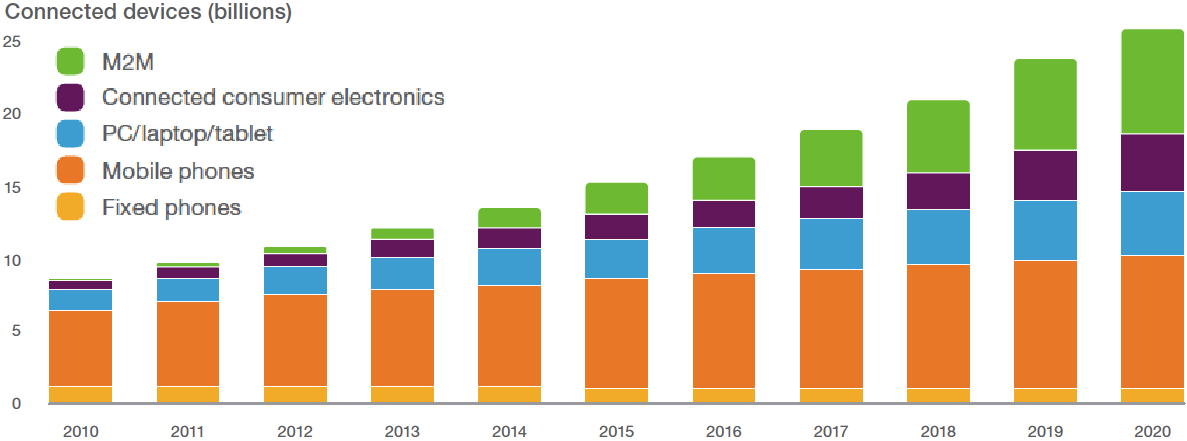
\includegraphics[width=\columnwidth]{figure/connected_devices.png}
\caption{Ericsson Mobility Report June 2015 \cite{connected_deveices} \label{ericsson_report}}
\end{figure}


%\section{Problem description}
RBS (Radio Base Station) is an integral part of the mobile data solutions delivered by Ericsson. A RBS consists of embedded components that are connected together in order to support high network availability to wide area network. A mobile network is a distributed system that consists of many RBSs. 
%Due to the fact that operators as well as subscribers expect that network services support almost everything in their daily life, so high availability of network services is an essential part in daily life. 
As long as network signalling volumes increase and operators demand more complex configurations for supporting more usage scenarios, the need for improving resilience is also increasing. The network should be flexible so that it responses to the challenge of the dramatic increasing in the network traffic and signaling created by the operators and subscribers~\cite{availability}.
%\newline

The Performance Management (PM) framework, one key component of RBS, is a framework used to count phone calls and network usages of subscribers. 
%Similarly to other components of RBS, the PM framework is tested using traditional approaches like unit testing and functional testing. % (mock testing~\cite{Mackinnon2001}). %; in this way %such 
%%software testing techniques are deterministic~\cite{deterministic}. 
%Unit testing %will not catch all errors in the code, since it cannot evaluate every execution path of the program. Unit testing 
%only tests the functionality of the units themselves, it will not catch integration or system-level errors. Although functional testing combines different test cases and tests the code at the system level, such a combination is usually limited. In fact, functional and unit testing approaches are deterministic~\cite{deterministic} and unknown failure modes % then random faults 
%are very hard to be detected. 
%%Therefore, there is a need of implementing a non-deterministic approach, fault injection approach uses random mechanism for detecting the unexpected faults at the same time can be utilized in large scale systems. So fault injection approaches can be complementary to the existing testing techniques. 
%%\newline
The RBS components, including the PM framework, are tested using traditional  approaches  like unit testing and functional testing.  Unit  testing  is the most adequate approach to test the functionality of the units taken individually, however it will not catch integration or system-level errors. Functional testing combines different test cases and can test the code at system level, however such a combination is usually limited. In fact, functional and unit testing approaches are deterministic and as such they mostly address failure modes that are expected. Potential unknown failure modes are very hard to be detected by traditional testing.

In order to catch also unknown failure modes, %do testing in a non-deterministic way,  
testing should be randomized and fault injection~\cite{nondeterministic} can be a valuable technique to be exploited for this purpose. 
While several approaches exist for fault injection, such as the already cited Chaos Monkey, they were not adequate for testing distributed embedded systems with very limited computational power such as the PM framework. This motivated the design and implementation of \approach{}. 
%which is specifically tailored for system with these characteristics: 
%%Some projects like Chaos Monkey use fault injection for online testing, but they were developed for testing distributed systems hosted on the cloud. Chaos Monkey is an open source project that has been developed by Netflix when they moved their data center to the cloud. The main function of Chaos Monkey is to inject random faults to the distributed system hosted on the cloud. 
%%%Fault injection is a popular technique for testing distributed systems, various researches on fault injection are springing out. At same time, other types of fault injection tools were also introduced, but most of them are used to test systems hosted on the cloud.  
%%RBS is a type of distributed system which consists of small embedded components. Previous approaches like Chaos Monkey are not feasible for such an embedded distributed system. Additional unavoidable requirements emerge for this type of systems, for instance: 
%limited computation and hardware capabilities, 
%%The new fault injection tool for such an embedded distributed system has new requirements; for instance the injection in the new fault technique is done 
%the fault injection must be done near to the hardware layer, %the programming language will be c++ instead of Java. On the other side, 
%the  fault injection technique must use shared libraries, %. Moreover, 
%the communication paradigm between the components should be inter-process communication.


%Each iteration was composed of four phases, namely:
%
%\begin{itemize}
%\item {\em Awareness of problem:} %collecting information about different fault types through deep literature studying. By studying the previous related work, we took an inspiration for developing the new approach. Furthermore, 
%we had weekly meetings with practitioners %the supervisors 
%at Ericsson organized by our industrial author in order to gather more information on how the system works as well as some suggestions about the injection. We also analyzed Ericsson PM framework documents for identifying the bottleneck of the system and determining the injections. Additionally, Ericsson's internal fault reports and other available documents helped in gathering more information about the weakness of the system and identifying where problems can occur. After deep studying of system weakness together with possible faults which might happen in reality, random faults were designed. At the same time the system was experimented by running with different scenarios and inspecting the log files. 
%\item {\em Suggestion and solution:} Based on Ericsson fault report and designed fault tolerant ability of the PM framework, potential fault types were discussed with practitioners. We decided to have two fault types, the first one was sending random messages and the second one was delaying messages. In sending random messages, we got the idea from the supervisor in order to test the filter ability of the PM framework against random invalid messages. Delaying the messages were performed between the critical components of the PM framework where faults can occur.
%\item {\em Implementation:} The implementation contains two steps: tool development and tool integration. The first step mainly concerns the work of development the fault injection tool using an Ericsson internal shared library called Inter Process Communication. The second step mainly concerns the work of integrating the developed tool into the automatic testing environment of the PM framework.
%\item {\em Evaluation:} 
%%Since we utilized agile development process, the fault injection approach was evaluated continually. Continuous evaluation of the approach helped us in developing the work as needed, decrease the uncertainty level, and increase the work quality. The source code of each iteration was pushed to the remote repository where the supervisor had access to it. During the weekly meeting with practitioners, we got feedback on the fault injection tool. Furthermore, we presented the fault injection tool after the last iteration to the development team and got some feedback from them. 
%\end{itemize}


%\section{Motivation}
%Services running in distributed systems are difficult to be tested using traditional methods \cite{FaaS}. When faults occur in running services, faults can exponentially propagate \cite{verification_testing}. In this case, identifying faults in a running application in a production environment would go a long way. Testing in large scale distributed system is very hard due to the fact that the number of faults that can occur at any time is very large as well as it is very hard to imagine the scenarios that can accrue. Traditional testing techniques are not sufficient to predict the effects of faults on realistic applications running on large distributed systems \cite{FaaS}.
%\newline



\section{Related Work}\label{sec:relatedWorks}
%This section describes the background of this thesis and some previous related work that aimed to provide fault injection approaches as well as implementations of fault injection tools.

\subsection{Fault injection}

%A software system does not always behave as it is expected. The more distributed system grows the more it suffers from different dependability issues for instance in embedded flight software, the presence of faults affects its dependability and can even have a big impact on the entire mission. Fault avoidance, fault removal and fault tolerance techniques are used for achieving high dependability. For preventing and minimizing the faults, faults removal and tolerance should be adapted in all software development stages staring from the design and implementation and ending with the verification and validation\cite{criticalsys_dep}. Dependability is an important issue especially when the software is critical safety system, faults can propagate and have a  consequent impact on the rest of the components. Furthermore service availability is also a very important aspect nowadays especially when the society becomes more Internet society \cite{availability}. Fault injection has been widely used in order to verify and validate the dependability and the availability of the software system. 

%Fault injection techniques are mainly used late on the development cycle after the software has been developed; there are some limitations when utilizing the fault injection in an early stage presented in \cite{rana2013improving}. To come over those limitations fault injection shall be combine with other testing like mutation testing for adapting it in an early stage of the development process \cite{rana2013improving}. 

There are two types of fault injection: hardware and software fault injection~\cite{rana2013improving}. 
%\newline
In hardware fault injection  faults are injected at the physical level by controlling the parameters of the environment variables. In this case fault types can be like disturbing the power supply, voltage sags, heavy ion radiation and electromagnetic interference etc.~\cite{rana2013improving}. 
%\newline
In software fault injection a possible strategy to inject faults is to consider %this can be done by implementing 
different fault types such as register and memory faults, system overload, and missing, delayed and faulty  messages. Faults can be injected within the application, between the target and operating system or between the critical components in the system. 
Software fault injection techniques can be classified into two groups based on when and where the faults are injected: %the first one is 
compile-time and run-time faults. 
Faults can be triggered with different mechanisms, for instance time-out, exception, code modification, and sending different random messages~\cite{rana2013improving}.   

%\subsubsection{Failure Scenario as a Service (FSaaS)}

%A research of fault injection is described in 
The work in~\cite{FaaS} presents a new model called Failure Scenario as a Service (FSaaS). The main purpose of this model is to test the resilience of cloud applications. This can be done by monitoring the result of generating different failure scenarios on the cloud. Their main research focus is to investigate the impact of the failure on the jobs running in Hadoop for analyzing the MapReduce jobs. Hadoop is an open source software framework %written in the Java language. The main purpose of Hadoop is 
to process large distributed data set on huge computer clusters~\cite{hadoop}. MapReduce is an efficient model for processing and generating large data set that is running on the distributed system on computer clusters~\cite{mapreduce}.    
%\newline
A fault injection tool called AnarchyApe~\cite{AnarchyApe} was used to inject faults into Hadoop clusters. In order to evaluate the effects of individual faults and combinations of faults, some sample fault scenarios and different types of workloads were performed on different types of Hadoop jobs. As a result of their study, they discovered that the resulting behavior of the distributed system depends much on the fault types, combination of faults, job types, and the time when the faults are injected. %Furthermore, with traditional testing, it is very hard to test the reliability of running services on the cloud. In large system, the number of faults that can happen are relatively large and therefore it is hard to test large scale system. 
The study presents a new model that can deal with large cloud applications to be tested efficiently. 
The model had helped them to identify the week spots of the system and trying to fix them as well as monitor the resources for efficient utilization.
%\newline
The limitation of the model is that it can be only used by cloud service providers and clients who rely on Hadoop. However, their goal is to develop a system that can be applicable to general cloud scenarios \cite{FaaS}. In this paper we aim at developing a fault injection approach and tool that can be applied to small embedded distributed systems. %Since embedded distributed systems are an essential part of most nowadays application, having an efficient tool for evaluating their robustness will be very beneficial and valuable.
 
%\subsubsection{Fault Injection and Mutation Testing with Model Based Development}
%
%A research of Increasing Efficiency of Verification and Validation by Combining Fault Injection and Mutation Testing with Model Based Development is presented in \cite{combinationtesting}. The main focus of this research is to proof that testing effectiveness and efficiency will be improved by applying fault injection techniques combined with a mutation testing approach for verifying and validating the automotive software at the model level. The main improvements of such testing is to detect the faults early in the development cycle thus providing enough time to be aware of the defects as well as less cost to fix them. 
%%\newline
%
%ISO 26262 standard stated the requirements for using the fault injection techniques. The study presented in \cite{combinationtesting}, describes that those requirements are challenging due to the fact that they are related to complete functionality rather that components of sub-component of the software. Considering that the fault injection techniques are used in the automotive at one electric component (ECU) or one software system, and seldom at the function level. Therefore, utilizing fault injection technique is not enough since fault injection techniques are used late in the development (when ECUs are being developed), and any detection of faults at this stage will be difficult and costly. 
%%\newline
%
%In the same study \cite{combinationtesting}, their research proposes a solution that the detection should be done at the model level when the ECUs functionality is still under design, in this case fault handling will be easy and cheap to resolve. Fault injection techniques are successfully used to detect the fault and identify the dependability problem of hardware and software when applied to complete system \cite{hsueh}. In order to increase the effectiveness of fault injection techniques and identify whether the fault should be injected at the model, software or ECU level, mutation testing should be utilized in order to verify the adequacy of the test cases. The combination of those approaches will improve the fault detection on an early design stage. A roadmap has been provided and described in \cite{combinationtesting}. The roadmap shows how a combination of fault injection and mutation testing approaches can be applied to modelling of automotive software for avoiding cost effects as well as increase the safety of modern and future cars. 
%%\newline
%
%The software development in the automotive industry and other similar industries widely adapted the paradigm of Model-Based Development (MBD) and the functionalities are safety critical functionality. MBD provides a significant functional testing in an early stage of the development process. Combination of fault injection and mutation testing approaches can be adapted to effectively verify and validate the functionality of the system. By detecting faults earlier, ability to perform much of verification and validation of the needed functionality and robustness the quality of the software will be exponentially improved. On the other hand, from this thesis we ensure that the cost for fixing the faults will be decreased when detecting faults in an early stage of the development cycle described in the discussion section "Quality of findings".    	

\subsection{Online Testing}
Because of the inherent complexity of modern systems, testing cannot be confined during development and offline phases but needs to be extended also to online phases. %, thus moving testing software engineers to users. 
%In fact, as one key method of ensuring quality of system, testing is needed during the whole life cycle of system. When software is delivered, testing is transferred from software engineers to users. Some people even think each using of system is one testing to the system [3]. In recent years, service has been thought as the goal of software. ?Software as service? is becoming one important common sense. And focuses on QoS (quality of services) are strengthened. As a result, focuses on online testing emerged and flourish in many areas[4], [5], [6], [7].
Several online testing approaches have been proposed in many areas, like service choreographies~\cite{Ali2014,Bertolino2012} ~\cite{Seaman2008,Binder1994,Wang2002,Canini2011}. %\pat{extend}


\subsubsection{Chaos Monkey Testing}

Chaos Monkey Testing (CMT)\footnote{\url{http://techblog.netflix.com/2012/07/chaos-monkey-released-into-wild.html}} %~\cite{FaaS} 
has been developed when Netflix moved their data center to Amazon Web Services (AWS). The main reason of developing CMT was to assess how potential failures in AWS would affect their ability to produce continuous services. 
%Netflix has a big challenge to maintain a continuous testing to their service reliability when they move their data center to AWS, in order to evaluate how potential failures in AWS would affect their ability to provide continuous services. They 
%The basic idea was to introduce failures to the system and stress it in order to investigate how the system acts, where does it fail, when it fails, and under which circumstances~\cite{FaaS}.
%\newline
%This paper has shows that the more types of fault injected, the more errors discovered. the fault injection has been shown well preperation on  how the algorithms works. Faults can easily propagate in large scale distributed system, especially on a system that has high dependencies between its components.  
%\newline
CMT works by sending fault commands to the components that are hosted in the cloud. On receiving the commands, the instance of the cloud itself will fail. By introducing faults CMT enables Netflix to discover the bottlenecks and weaknesses in their systems. Moreover, this helps them to strength the weak areas that are critical in their system. As a result of their study, they have discovered that CMT helps to detect different failure scenarios and to find %. CMT helps to find 
unexpected failures that cannot be detected using traditional methods. %consequently, CMT helps in building a robust system that is resilient against failures.
%\newline

CMT software design is flexible and can be used for other cloud service providers. However, it is just applicable for testing the availability and robustness for the services running in the cloud. Chaos Monkey Testing is not be applicable in traditional systems with a small number of complex tasks or threads, since this can lead to complete failure within a short time. Chaos Monkey is more applicable to a large scale system that has the ability to perform even in the presence of failures. %Instead, LiC only triggers the monitoring process, then fast replacement of the terminated software part can be performed. 
Additionally, CMT suffers from the limitation in terms of computational power. In the case of a large number of test cases to be executed, it might even dominate the power consumption. Using CMT in large scale systems will be costly and will consume extra resources such as network bandwidth, storage space, and processing power~\cite{gunawi2011failure}. When using this approach, an engineer should consider hardware reliability, memory managements, and the running environment. 
 
\subsubsection{Let it Crash Philosophy}
The work in~\cite{woskowskiassessing} investigates the use of the Let-it-Crash (LiC) paradigm to assess the applicability for safety related software, check how error handling perform, as well as identify potential improvements for future work. %Erlang is the programming language used. %was used as an implementation language for safety related functionality~\cite{woskowskiassessing}. 
%\newline
The main challenge of the LiC paradigm is to identify different software fault types in order to improve error handling in safety critical systems. 
%\newline
 
%%The evaluation of the LiC approach mainly depends on how well the system meets those requirements and does the system acts as it is expected. 
%The following assumptions acted as requirements for developing flexible software architecture that can manage different fault scenarios and at the same time for assessing the applicability of  LiC: 
%%\begin{itemize}
%%  \item 
%(i) Ensure the execution of critical functions; 
%%  \item 
%(ii) Prevent the unintended execution of a function; 
%%  \item 
%(iii) Define and monitor the conditions for carrying out a critical function; 
%%  \item 
%(iv) Ensure carrying out critical functions at a specific time and in a specific order; and 
%%  \item 
%(v) Unexpected failures either have no influence or result in a safe state.
%%  \end{itemize}
 
%Chaos Monkey Testing is not be applicable in traditional system with a small number of complex tasks or threads, since this can lead to complete failure within a short time. Chaos Monkey is more applicable to a large scale system that has the ability to perform even in the presence of failures. Instead, 
LiC only triggers the monitoring process, then fast replacement of the terminated software part can be performed. 
%\newline
LiC can be efficiently utilized in safety related software development that have low number of complex tasks. The programming language should be Erlang and it does not cover large scale embedded distributed system. Furthermore, this approach has a problem when it comes to safety-critical system with hard time constraints, since Erlang is not supporting that~\cite{woskowskiassessing}. 


%\newline


%\subsection{Improving Fault Injection in Automotive Model Based Development}
%
%Model based development (MBD) has been widely used in the automotive software development. MBD allows the verification and validation of the functionality and their dependencies in an early stage of the development cycle. Fault injection can be used for dependability evaluation at the model level for the hardware artifacts. However, the interdependencies between the system and its environment at the model level may affect the result reliability to be unrealistic. This research paper presents an approach in order to come over this problem that they observed. This problem makes it difficult to utilizing fault injection at an early stage of development. Fault the bypass modeling (FBM) framework has been presented and evaluated in \cite{rana2013improving}. The FBM framework can be used in order to observe the system behavior under fault injection modes. With this framework the system behavior will be monitored and analyzed in an early stage of the development cycle.
%%\newline
%
%Analyzing system behavior in an early stage will reduce the amount of defects in late stage, improve the quality, as well as reduce the development time. Those advantages are very important especially when the system is safety critical system. Fault injection techniques have been proven to be an efficient technique for testing the robustness of the system. However, fault injection has a limitation when using it in a close loop model testing, the reason behind that is the interdependences between the system and its environment at the model level may affect the result to be unrealistic with unrealistic system behavior. Using the FBM will resolve this problem thus make it possible to use fault injection correctly in order to test the behavior model for dependability and robustness evaluation. The FBM helps an early defect detection which will not only save time and cost, but also will increase the quality of the development. Using the fault injection techniques at the model level will allow discovering the dependability issues on an early stage. As a conclusion more robust system will be developed an evaluated continuously from the early stage \cite{rana2013improving}. 


\section{Fault injection approach}\label{sec:approach}

%The approach we present in this paper 
\approach{} uses fault injection at run-time to test distributed embedded systems with very limited computation power. 
%Chaos Monkey Testing~\cite{FaaS,gunawi2011failure} and the Let-it-Crash paradigm~\cite{woskowskiassessing} are important related works, however, as mentioned before and further discussed in Section~\ref{sec:relatedWorks}, the characteristics of our target systems hamper their use in this context. 
Section~\ref{sec:researchMeth} presents the adopted research methodology, and Section~\ref{sec:approach_approach} presents an overview of the \approach{} approach. 

%This work has been developed in collaboration with a team within Ericsson AB in Gothenburg, Sweden. %\pat{add more details about the team within Ericsson}
%Due to the complexity of distributed systems and the challenges of testing distributed systems with traditional approaches, a new approach based on some existing distributed systems testing technique and researches is needed. %The main investigation of this thesis is how to develop a new fault injection approach and implement a new fault injection tool to help the development team at Ericsson in testing their embedded distributed system. Moreover, we aim to make the fault injection approach as general as possible so it can be used in other companies and bring benefits to the embedded industry in general.
%\newline
%As anticipated in the introduction t

\subsection{Research methodology}\label{sec:researchMeth}

Our collaboration model between academia and industry is based on the 
design and creation methodology, which was developed to address theoretical questions about the nature of learning
in context. It is mainly used when a creation of new knowledge is seeking in
order to solve a particular phenomenon through designing innovative artifact~\cite{ResMethod}.

The \approach{} approach and tool have been conceived and implemented following an agile development process %iteratively in four iterations 
and in strong synergy with practitioners within Ericsson. 
As anticipated in the introduction the approach and tool have been developed in four iterations and each iteration was composed of four phases, namely: 
\begin{itemize}
\item{\em Awareness of problem}: %collecting information about different fault types through deep literature studying. By studying the previous related work, we took an inspiration for developing the new approach. Furthermore, 
%basically through 
we had weekly 
meetings with practitioners %the supervisors 
at Ericsson and we analysed available documentation about the PM framework 
%organized by our industrial author 
%in order to gather more information on how the system works as well as some suggestions about the injection. We also analyzed Ericsson PM framework documents 
for identifying the bottleneck of the system and determining the injections. Additionally, Ericsson's internal fault reports and other available documents helped in gathering more information about the weakness of the system and identifying where problems can occur. 
%After deep studying of system weakness together with possible faults which might happen in reality, random faults were designed. At the same time the system was experimented by running with different scenarios and inspecting the log files. 
\item 
{\em Suggestion and solution}: based on Ericsson fault report and designed fault tolerant ability of the PM framework, potential fault types were discussed with practitioners. We decided to have two fault types, the first one was sending random messages and the second one was delaying messages. The rational of sending random messages is to 
%, we got the idea from the supervisor in order to 
test the filter ability of the PM framework against random invalid messages. Delaying the messages were performed between the critical components of the PM framework where faults can occur.
\item 
{\em Implementation}: the implementation contains two steps: tool development and tool integration. The first step mainly concerns the work of development the fault injection tool using an Ericsson internal shared library called Inter Process Communication. The second step mainly concerns the work of integrating the developed tool into the automatic testing environment of the PM framework.
\item 
{\em Evaluation}: since we followed an agile development process we had a continuous evaluation of the approach and tool through these means: %
%\begin{itemize}
%    \item 
(i) we had weekly meeting with practitioners for getting feedback;
    %\item Well identified requirements for the expected conformance level on how the tool should work.
%    \item 
(ii) continuous validation of  defined requirements for the expected conformance level on how the approach should work; 
%    \item 
(iii) observation of the results of the execution of the fault injection tool stored in log files;
(iv) comparison of the observed results with the expected ones (how the system should perform in its normal state);
%    \item 
(v) if faults were detected, evaluation of the faults by tracing back to the cause that made them.
%\end{itemize}  
\end{itemize}

\subsection{The \approach{} approach}\label{sec:approach_approach}

\begin{figure}[h]
\begin{center}
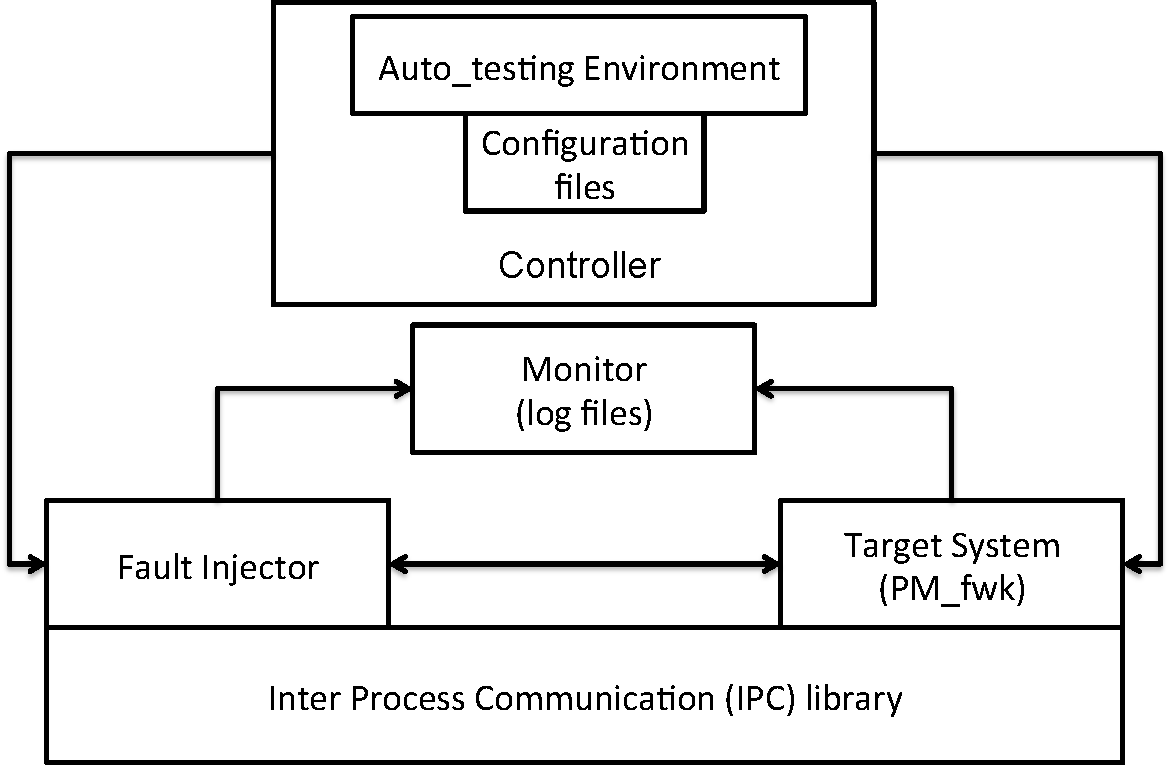
\includegraphics[width=\columnwidth]{figure/faultInjectionApproach.pdf}
\caption{The \approach{} approach \label{Fualt_injection_Model}}
\end{center}
\end{figure}

Figure~\ref{Fualt_injection_Model} presents the basic components of \approach{}. It consists of the target system (PM\_fwk), fault injector, monitor (log files), Inter Process Communication (IPC) library as well as the controller that has the automatic testing and the configuration files.
As better explained in Section~\ref{sec:implementation} configuration files are exploited to make the fault injector customizable, extensible, and reusable in different contexts.

After running the \approach{} tool all data are monitored from the log files using stack trace. These data are collected and analyzed for the evaluation of the approach and of the tool. % as well as for answering the main research questions. 
The user can run and control the tool through the controller, where the automatic testing environments and the configuration files are located. Through the automatic testing environment different testing techniques are listed. The \approach{} tool supports random mechanisms where the number of faulty messages, message delay, and the time interval between sending the messages are randomized. The user can manually adjust the test cases through the configuration files.    

The \approach{} approach provides different fault types at different location and time. We have developed two fault types: (i) sending random messages and (ii) delaying the messages. Fault types such as sending invalid messages and delaying the messages were done by linking some dynamic libraries of IPC during run time. IPC library is a separate component, which consists of different system functionalities such as sending the messages between different system component. After deep study of the PM framework documentation and discussion with the practitioners, system targets were identified. The system targets were some critical components of the PM framework that have strong dependencies. Faults were injected on system targets that have strong coupling. Due to the fact that time factor can have an effect on running the experiments and to make sure that the result we got are reliable, we have repeated the experiments at different time. For non deterministic testing, as pointed in~\cite{testselectionnondeterministic}, as long as the number of the repetition of test sequence increases, the quality of testing will also be increased. %In actual testing this number is limited due to economical and practical reasons. However, when executing the testing large number of time, the probability that all possible execution paths are executed will be reasonably high.  

\subsubsection{Sending random messages}
The communication within the system follows some specific protocols.  Sending random messages is mainly developed to test the fault tolerance ability of the protocols. The messages are categorized into three types: request, confirmation, and rejection.  Based on the designed fault tolerance feature and the possible message types in reality, we only perform sending of random request messages. We focus on three aspects of the invalid messages, the origination, the contents and the amount of sending.

The system is designed to tolerate invalid request messages, one main filtering standard of invalid messages is the origination of the messages. We focused on three aspects of the message origination, the namespace name, the mailbox name and combination of namespace and mailbox names. We first created multiple mailboxes which have the same namespace name, this means that the random messages are generated from different threads but the same process. Then we created mailboxes with same mailbox names but different namespace names; this means that the random messages are generated from both different threads and processes. Lastly, we created mailboxes with both different mailbox names and namespace names. Three cases of mailbox and namespace names are shown in Table~\ref{table:4.1}.

\begin{table}[ht!]
\centering
\begin{tabular}{| c | c | c |r}
 \cline{1-3}
       & mailbox & namespace \\ 
 \cline{1-3}
 case 1 & S & D & \hspace{1.3cm} S stands for same\\ 
 \cline{1-3}
 case 2 & D & S & D stands for different\\ 
 \cline{1-3}
 case 3 & D & D & \\ 
 \cline{1-3}
\end{tabular}
\caption{Combinations of mailbox and namespace names} %, S means same, D means different}
\label{table:4.1}
\end{table}

The message contents inside the system varied dramatically: some contents describe the actual payload, some describe the protocol version, some specify the size of the messages. The fields of the messages were also different from each other. Based on the above characteristics, we constructed the random messages from two different aspects, random fields and random contents. 

The amount of random messages would affect the filtering ability of the protocols. For instance, by sending one random message, the system is able to filter it, but by sending 1000 random messages, the system might only be able to filter 500 of them. With a huge amount of random messages, the CPU load of the systems would be high. 

\subsubsection{Delaying messages}
The second fault injection scenario was delaying the messages between the system components. The delay mechanism used default and randomize time interval between different components on the system in order to check if the system can handle different timeout intervals. There are multiple types of messages sending within the PM framework, e.g., request message, response message, rejection, confirmation message and messages describing the data. Some types of messages followed some time out mechanism strictly. For instance, when the connection request is sent, the node waits for confirmation or rejection messages for a period of time; if neither a confirmation nor a rejection message is received, the current request of the node just goes in timeout. 

\begin{figure}[hh!]
\centering
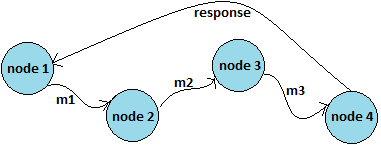
\includegraphics[width=.7\columnwidth]{figure/chaningMSG.png}
\caption{Message delaying chain \label{chaning}}
\end{figure}

Some messages sent within the PM framework have relationships with each other. Those messages usually work as a chain, as shown in Figure~\ref{chaning}. In this case, \texttt{node1} sends a request to \texttt{node4} for some data, and at the same time a clock starts for the time out mechanism. In order to receive the data, some messages are sent to \texttt{node2} and \texttt{node3}, but \texttt{node1} only waits for a response from \texttt{node4}. Delaying can happen on any of the messages sent between \texttt{node1} and \texttt{node4}. In reality, such a chain can be really long and the delay of the messages sent between each nodes can also be very unpredictable.

Delaying messages in the PM framework also tests the network performance of the framework. %By delaying messages in the PM framework, the network performance of the PM framework is tested. 
Currently the PM framework network performance test is conducted by adjusting the network bandwidth. This approach has two main drawbacks. First, the test has some hardware requirements, which makes the test more complicated. Second, adjusting the network bandwidth makes the test uncontrolled, because the delaying of the message caused by a low network bandwidth is very hard to track. The current network performance test is like a black-box testing, since what is really going on in the system during the test is not peered. Our test provides a white box testing for the PM framework network performance. During the message delaying, each message delaying is recorded in the log file, and then the PM framework developers at Ericsson can easily track the message delaying. A future network bandwidth benchmark has been created based on the experiences of the message delaying.


\section{Implementation}\label{sec:implementation}

The implementation consists of two steps: tool development and tool integration. The first step mainly concerns the development of the fault injection tool using an Ericsson internal shared library called Inter Process Communication (see Section~\ref{sec:IPC}); the results of this step are some compiled C++ object files. The second step mainly concerns the work of integrating the developed tool into the automatic testing environment of the PM framework, where Shell Scripts and Ruby were used (see Section~\ref{sec:PM}). Then, this section will describe the implementation of the procedure for the two fault types we considered in the study: sending random messages (see Section~\ref{sec:sendingRandomMessages}) and delaying messages (see Section~\ref{sec:delayingMessages}).

\subsection{Inter Process Communication}\label{sec:IPC}
Inter Process Communication (IPC) is used as a communication paradigm in some components of the PM framework. Collection of information from the system is done by handling the collection of the counters and events between its components. %\cite{pmf}.
 IPC is used to send messages between mailboxes, processes, and processors. A processor is an execution unit that is handled by one instance of an operating system, it can have multiple cores and several simultaneously executing contexts. A process has its own memory map and can have several running threads. A thread is a single execution context that can coexist with other threads within a process. We worked on a simulated environment, where the processor was the CPU of the computer, a process was a simulation of a processor on the embedded components,  and a thread was a simulation of a process in the real operating system. Figure~\ref{simulationVSembedded} shows the relationship between the real operating system and the simulated environment. In our implementation, only processes and threads were involved, they were identified by the process namespace and the thread name. %Both the namespace and the thread name have human readable names.
%\newline

\begin{figure}[h]
\centering
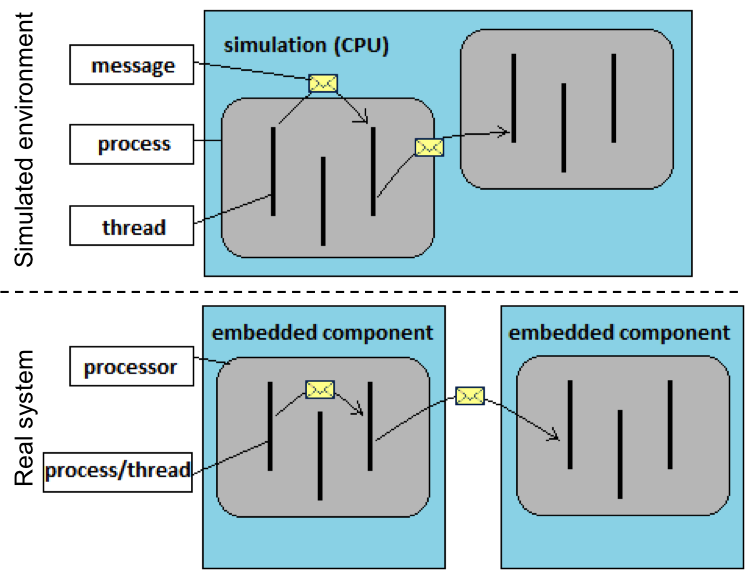
\includegraphics[width=\columnwidth]{figure/simulationVSembedded.png}
\caption{Relationship between real system and  simulated environment \label{simulationVSembedded}}
\end{figure}

IPC is a widely used library of RBS. The PM framework is built on top of IPC, it uses the APIs of IPC for the communication within the system. Based on this feature, we started our implementation without touching the code of the PM framework; instead we used the IPC APIs. In this way, we are able to inject random faults into the PM framework from outside the framework, and therefore that there is no need of extra computation for the framework to cater for fault injection. %This is a key difference with respect to Chaos Monkey Testing.

\subsection{Automatic testing environment}\label{sec:PM}
We developed a set of automated scenarios %that test the PM use cases that operation in reality
%In order 
to test the functions of the PM framework %, a set of automated scenarios that test the PM use cases that operation 
when operating in reality. % have been developed. 
The automatic testing environment is used to test the PM framework with such scenarios. The automated test scenarios will be used by the fault injection tool to verify that the PM works even in the presence of faults. 
%\newline

The \approach{} tool was integrated into the automatic testing environment using Shell Scripts, which injects random faults into the PM framework while running with the scenarios. The automatic testing environment also controls the operations of the fault injection tool like code generation, compiling and linking. The integration of \approach{} with  the automatic testing environment enhances the adoptability in industry and the usability of the tool.

%By integrating the tool into the automatic testing environment, the operation of the fault injection tool is more user-friendly and errors are more likely to be detected. 

The running results of fault injection are presented in the end of the automatic testing environment and traced in different log files. Figure~\ref{terminal} shows one type of running results in the end of the automatic testing environment, where the errors and corresponding log files are presented.
%\newpage

\begin{figure}[!ht]
\centering
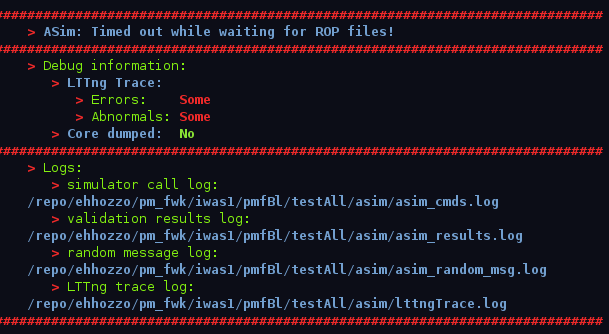
\includegraphics[width=\columnwidth]{figure/terminal.PNG}
\caption{Running results of automatic testing environment \label{terminal}}
\end{figure}


\subsection{Sending random messages}\label{sec:sendingRandomMessages}
In IPC, different messages were constructed with C++ structs; after initialization, the message objects were encapsulated in a message union and sent together. The fields of the messages are specified in some XML files; an excerpt is shown in Listing~\ref{xml_code}. We first ignored those files and constructed the messages with random fields, this means that the messages might miss some necessary fields and might contain some extra unnecessary fields. After that we constructed the messages following the XML files but with randomly filled contents, for instance, making the field called messages size to be a random number instead of the real message struct.         
%\newline                                              

\begin{minipage}{.96\columnwidth}
\lstinputlisting[
    language=xml,
    firstline=1,
    lastline=4,
    firstnumber=1,
    caption={XML that specifies message fields},
    label={xml_code},
]
{code/xml.xml}
\end{minipage}

Constructing the message structs was based on the skeleton of the XML files, different categories of messages had different message fields and required different C++ header files. In order to implement the randomization mechanism, all the request message structs and their corresponding required header files need to be considered. %The existing request messages might change in the future. 
To make the functionality of sending random messages customizable, 
%, to make the messages which were to be sent controllable, 
the message are specified in a configuration file. A code generator written in Ruby is used to create the message structs. By reading the configuration file and the XML file that specifies the message fields, different message structs code are generated and compiled to different binaries. 
%\newline

The next step after the construction of random messages is %being constructed, the next step was 
to create the senders. The senders are actually some mailboxes located in the same namespace, which means that each mailbox has a separate thread and they are all located in the same process. In order to send the messages to some targets, the mailbox address of the targets should be known. In the PM framework, the mailbox addresses can be located by using combinations of the namespace names and the mailbox names. In our implementation, we put all the namespace names and mailbox names into vectors, we calculate 
%tried to locate 
all possible combinations and we put them into a map.  %as shown in Listing~\ref{locate_code}. 
So if there are $n$ namespace names and $m$ mailbox names, then we have $m*n$ combinations in total. Once a TID\footnote{TID stands for Thread ID, i.e. an identifier used to identify a thread. It is also used to identify the mailbox associated with that thread.} is successfully located, it is saved in another vector which will be used as the target to send. The messages are sent in two different ways, synchronously and asynchronously. Sending the messages synchronously is  implemented by joining the mailbox to the main thread.  
%\newline

%\begin{minipage}{.96\columnwidth}
%\lstinputlisting[
%    language=C++,
%    firstline=1,
%    lastline=9,
%    firstnumber=1,
%    caption={Code that creates all combinations of namespaces and mailboxes},
%    label={locate_code},
%]
%{code/code2.cc}
%\end{minipage}

Sending random messages is integrated into the automatic testing environment, which is written in Shell script. Every error triggered by the random messages is logged and the logging is implemented with a watch dog. The watch dog keeps track of which message are sent and how many of them were sent. The watch dog also keeps pinging all the previously located TIDs and if any of them crashes during the time when the messages are sent, the watch dog would also log such a TID. The log file provides a summary of all the relevant events happened while injecting random messages to the PM framework; this facilitates the detection of errors that are not found with unit testing.

\subsection{Delaying messages}\label{sec:delayingMessages}
The message sending of the PM framework uses IPC by linking some dynamic libraries during run time. In C and C++, it is possible to wrap the dynamic library functions. Such a wrapping is implemented by creating shared libraries that override the functions of the original dynamic libraries. Such a dynamic library file can be linked by setting an environment variable called \texttt{LD\_PRELOAD}. We implemented the delaying messages by wrapping the IPC dynamic libraries that are responsible for sending messages. As shown in Listing~\ref{wrap_code}, the name of original message sending function was called  \texttt{\_\_itc\_send}, the main parameters of this function were the message contents named ``{\em msg}", the receiver named ``{\em to}" and the sender named ``{\em from}". The wrap function had exactly the same function name and parameters with the original function. 
%\newline

\begin{minipage}{.96\columnwidth}
\lstinputlisting[
    language=C++,
    firstline=1,
    lastline=16,
    firstnumber=1,
    caption={Code that wraps the sending function of IPC},
    label={wrap_code},
]
{code/code.cc}
\end{minipage}


%At Line 13, a function called ``{\em dlsym}" took a handle of the dynamic library which contains the \texttt{\_\_itc\_send} function, this handle was returned to a function pointer called \texttt{\_\_real\_itc\_send}, which has the same parameter types as the original \texttt{\_\_itc\_send} function. By calling the \texttt{\_\_real\_itc\_send} function with the original parameters of \texttt{\_\_itc\_send}, the original \texttt{\_\_itc\_send} got called. But 
As can be seen in Line 14,
before calling \texttt{\_\_real\_itc\_send}, we let the current thread sleep for 1 second; % as shown at Line 14, 
this means that the \texttt{\_\_itc\_send} function was always executed 1 second after being called, which implemented the delaying of message sending.
%\newline

\begin{minipage}{.96\columnwidth}
\lstinputlisting[
    language=xml,
    firstline=1,
    lastline=5,
    firstnumber=1,
    caption={XML for setting the environment variable},
    label={envconfig_code},
]
{code/env_config.xml}
\end{minipage}
%\newline

After being compiled, the shared library can be loaded by setting the environment variable \texttt{LD\_PRELOAD} to the path of this shared library. %The nodes of the PM framework are started with an Erlang shell, which is different from a normal Linux shell. 
The environment variables are set in an XML file as shown in Listings~\ref{envconfig_code} and~\ref{env_code}. At Line 4 of Listing~\ref{envconfig_code} the environment variable called \texttt{LD\_PRELOAD} is set to the path of a shared library file called ``wrap.so". Listing~\ref{env_code} is an XML configuration file of a node in the PM framework, Line~5 contains the path to the environment variable configuration file, the environment variable is set by adding this line into the node configuration file and restarting the node.
%\newline



\begin{minipage}{.96\columnwidth}
\lstinputlisting[
    language=xml,
    firstline=1,
    lastline=7,
    firstnumber=1,
    caption={XML configuration file of a node in the PM framework},
    label={env_code},
]
{code/env.xml}
\end{minipage}
\section{Validation and Results}\label{sec:results}
This section introduces the results of performing fault injection with the \approach{} %fault injection 
tool. First, we show the steps of performing the fault injection, the variable parts, and the expected outcomes. Then, we show the real outcome, the performance of the PM framework and the detected bugs.

%Design and creation research methodology was selected for creating the fault injection approach. Design and creation methodology is used for investigating a certain phenomena by creating and designing a new artifact. The phenomena in this study is to test the robustness of the embedded distributed systems and the artifact is the fault injection approach.  

%Agile development process was utilized for creating the fault injection approach. Fault injection tool developed in four iterations. Random sending messages was implemented in the first iteration, then we integrated the random messages sending into the automatic testing environment in the second iteration. Messages delaying was implemented during the third iteration and was integrated into the automatic testing environment in the last iteration.  

As anticipated in the introduction, we developed the approach through an iterative approach. In order to evaluate if the fault injection approach reached the conformance level against its requirements, the approach was evaluated at the end of each iteration. 
The evaluation was done by comparing the results of running the tool and the expected ones. At the end of the final iteration, we made a final validation. 
%conclusion was built on how well the approach worked. Final evaluation of the developed approach described at the result part in details, we could see that 
The fault injection approach has detected unexpected fault that were not seen on the previous testing techniques. As matter of fact, we could also see that this approach is able to identify the bottleneck of existing embedded distributed systems.  In the following we report detail results of the validation. Specific details are however omitted according to non disclosure agreements with the company.


\subsection{Sending random messages}
%The communication within the system follows some specific protocols.  Sending random messages is mainly developed to test the fault tolerance ability of the protocols. The messages are categorized into three types: request, confirmation, and rejection.  Based on the designed fault tolerance feature and the possible message types in reality, we only perform sending of random request messages. We focus on three aspects of the invalid messages, the origination, the contents and the amount of sending.
%
%The system is designed to tolerate invalid request messages, one main filtering standard of invalid messages is the origination of the messages. We focused on three aspects of the message origination, the namespace name, the mailbox name and combination of namespace and mailbox names. We first created multiple mailboxes which have the same namespace name, this means that the random messages are generated from different threads but the same process. Then we created mailboxes with same mailbox names but different namespace names; this means that the random messages are generated from both different threads and processes. Lastly, we created mailboxes with both different mailbox names and namespace names. Three cases of mailbox and namespace names are shown in Table~\ref{table:4.1}.
%
%\begin{table}[ht!]
%\centering
%\begin{tabular}{| c | c | c |r}
% \cline{1-3}
%       & mailbox & namespace \\ 
% \cline{1-3}
% case 1 & S & D & \hspace{1.3cm} S stands for same\\ 
% \cline{1-3}
% case 2 & D & S & D stands for different\\ 
% \cline{1-3}
% case 3 & D & D & \\ 
% \cline{1-3}
%\end{tabular}
%\caption{Combinations of mailbox and namespace names} %, S means same, D means different}
%\label{table:4.1}
%\end{table}
%
%The message contents inside the system varied dramatically: some contents describe the actual payload, some describe the protocol version, some specify the size of the messages. The fields of the messages were also different from each other. Based on the above characteristics, we constructed the random messages from two different aspects, random fields and random contents. 
%
%The amount of random messages would affect the filtering ability of the protocols. For instance, by sending one random message, the system is able to filter it, but by sending 1000 random messages, the system might only be able to filter 500 of them. With a huge amount of random messages, the CPU load of the systems would be high. Therefore, t
The validation related to random messages wants to give an answer to these questions: 

 \begin{itemize}
 \item {\em Is the system still able to filter invalid messages?} 
 \item {\em Does a high CPU load affect other parts of the system?} 
 \end{itemize}
 
 To answer the above two questions, we sent random messages in two ways, synchronously and asynchronously.
Filtering of invalid messages is conducted by checking the properties of the messages. Such checking consumes time and processing power. So the filtering ability can also be affected by the frequency of the random messages. To test the filtering ability of the PM framework in terms of random message frequencies, the random messages are sent to the PM framework with different frequencies. This was implemented by giving different time intervals between each message sending. 

The number of invalid messages that need to be generated in order to let the system behaves differently varies depending on the time interval between the messages as well as the time when the messages are triggered. Sending a lot of invalid messages without having any time interval between messages leads the system to not behave as expected. This happens due to the fact that the computation power of the embedded components is limited, the number of the messages are large and there is not enough time between message sending. Thus, the system will not be able to recognize if the message is valid or not. 

\begin{figure}[h!]
\centering
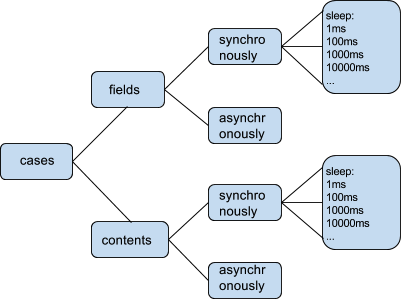
\includegraphics[width=.8\columnwidth]{figure/testingchain.png}
\caption{Testing chains \label{testingchain}}
\end{figure}

Figure~\ref{testingchain} shows the test chains of the PM framework. One sample test chain from the left to right can be read like this: test case1, with same fields but different contents, send the random messages synchronously, the time interval between each random message is 100ms. In order to perform the test randomly, we created different C++ classes to represent different variables in the chain. When the test starts, variable objects of the test chains are initialized and connected randomly. There are four variable classes, which are Cases, DataType (fields or contents), Concurrency (synchronously or asynchronously), and Intervals.

By performing the random message sending to the PM framework, we are able to test the PM framework according to two different aspects. The first aspect is the message type, which tested the PM framework at functional level. The second aspect is the message amount, which tested the PM framework at the performance level. The module test of the PM framework has covered almost all the invalid message sending, but the test is not random and the messages are sent one at a time. Our test sends random messages randomly and messages are also combined randomly. This helps the PM framework developers at Ericsson finding many corner cases that were not covered before. %which the module tested does not cover. 
The random messages sending also plays a performance test role. By adjusting the number of random messages and the time interval between the random messages sent, a performance threshold of the PM framework was found. Based on the demand in reality, this test helped the PM framework developers finding secure hardware requirements, which provide optimal and economic solutions for Ericsson.

\begin{figure}[h!]
\centering
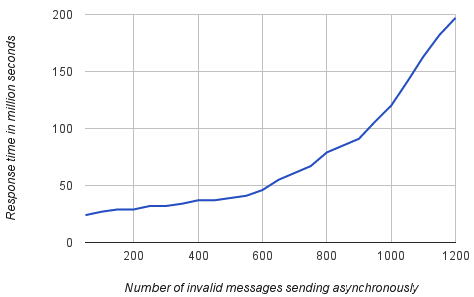
\includegraphics[width=\columnwidth]{figure/asynseding.png}
\caption{Sending invalid messages asynchronously \label{asynseding}}
\end{figure}

Figure~\ref{asynseding} shows a snapshot of sending random messages to one node in the PM framework. The response time of messages sent to this node should be less than 200 milliseconds, if the there's no response after 200 milliseconds, the sender will timeout. Figure~\ref{synchsending} shows a snapshot of sending random messages synchronously with different time intervals between each sending which will not trigger timeout. Figure~\ref{asynseding} shows that the node can maximally receive 1200 random messages at the same time. Figure~\ref{synchsending} shows that in order to send 6000 messages, each message sending should have at least an interval of 80 milliseconds. These snapshots have been saved as benchmarks for improving the performance of the nodes.


\begin{figure}[hh!]
\centering
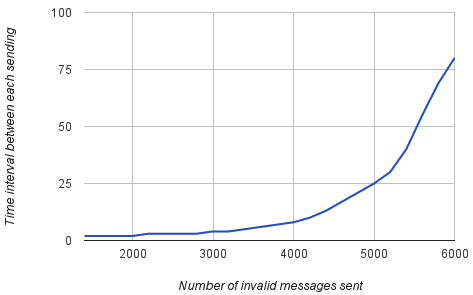
\includegraphics[width=\columnwidth]{figure/synchsending.png}
\caption{Sending invalid messages synchronously \label{synchsending}}
\end{figure}

Thanks to this tests we identified some errors that where not identified by traditional testing. For instance fuzzing of signals has detected a weakness in handling dynamically sized objects causing a crash which then could be rectified.

\subsection{Delaying messages}
%The second fault injection scenario was delaying the messages between the system components. The delay mechanism used default and randomize time interval between different components on the system in order to check if the system can handle different timeout intervals. There are multiple types of messages sending within the PM framework, e.g., request message, response message, rejection, confirmation message and messages describing the data. Some types of messages followed some time out mechanism strictly. For instance, when the connection request is sent, the node waits for confirmation or rejection messages for a period of time; if neither a confirmation nor a rejection message is received, the current request of the node just goes in timeout. 
%
%\begin{figure}[hh!]
%\centering
%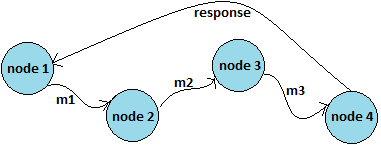
\includegraphics[width=.7\columnwidth]{figure/chaningMSG.png}
%\caption{Message delaying chain \label{chaning}}
%\end{figure}
%
%Some messages sent within the PM framework have relationships with each other. Those messages usually work as a chain, as shown in Figure~\ref{chaning}. In this case, \texttt{node1} sends a request to \texttt{node4} for some data, and at the same time a clock starts for the time out mechanism. In order to receive the data, some messages are sent to \texttt{node2} and \texttt{node3}, but \texttt{node1} only waits for a response from \texttt{node4}. Delaying can happen on any of the messages sent between \texttt{node1} and \texttt{node4}. In reality, such a chain can be really long and the delay of the messages sent between each nodes can also be very unpredictable.
%
%Delaying messages in the PM framework also tests the network performance of the framework. %By delaying messages in the PM framework, the network performance of the PM framework is tested. 
%Currently the PM framework network performance test is conducted by adjusting the network bandwidth. This approach has two main drawbacks. First, the test has some hardware requirements, which makes the test more complicated. Second, adjusting the network bandwidth makes the test uncontrolled, because the delaying of the message caused by a low network bandwidth is very hard to track. The current network performance test is like a black-box testing, since what is really going on in the system during the test is not peered. Our test provides a white box testing for the PM framework network performance. During the message delaying, each message delaying is recorded in the log file, and then the PM framework developers at Ericsson can easily track the message delaying. A future network bandwidth benchmark has been created based on the experiences of the message delaying.

In this case the validation wants to give an answer to the following question: 

 \begin{itemize}
 \item {\em Is delaying messages an effective strategy?} 
 \end{itemize}

\begin{figure}[hh!]
\centering
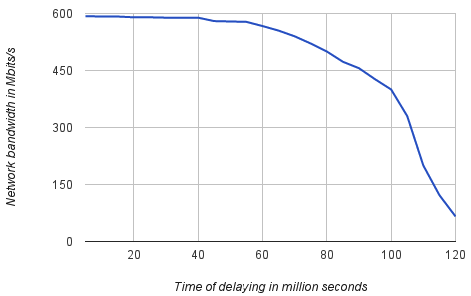
\includegraphics[width=\columnwidth]{figure/bendelay.png}
\caption{Message delaying and corresponding network bandwidth \label{bendelay}}
\end{figure}

In order to provide an answer to this question, we operated as follows. 
Figure~\ref{bendelay} shows the time of delaying in milliseconds and the corresponding network bandwidth in Mbit/s. The nodes use wireless communication and Ericsson uses the international standard of Wireless 802.11n~\cite{Wireless}, whose normal bandwidth is 600 Mbit/s. This benchmark is used to adjust the %when the performance test by adjusting 
network bandwidth when the performance is performing abnormally; the corresponding delaying will be run to check which process is responding slowly.

Randomized delays detect misconfigured timeout handling. This was not identified by manual testing since the manual test case had the same mistake of the production code, so it was missed. This testifies the potential existence of human bias in manual testing.

\subsection{Improvements to the software architecture}

Since the complexity of the software is dramatically increasing and systems are scaling over the time, the dependency level will also be increased. In a distributed system, there are always dependencies between the components and some dependencies are more critical than others. % on how the system should perform; t
This can be due to the fact that the amount of coupling between the components varies. In order to perform a particular action, the action should follow a specific sequence performed at different components that are connected with each other. Whenever a critical component has failed, the rest of the connected components can also fail. 

After a deep study of the distributed system architecture at Ericsson, we identified some critical components, which failures can be potential due to the strong dependencies. For such dependencies we used message delaying as failure type for testing the timeout mechanism. %is a potential failure type in such dependencies. 
Specifically, we delayed the messages between the critical components as well as tracked the system behavior through the log files. Under those circumstances, we have discovered that the system will not act as it should be when delaying the messages at a specific time. In the long run, software architecture can be improved by having lower dependencies on those critical components. By having lower coupling, components will be easier to replace, reduce the chance that a change in one component causes a problem in the other components which enhances reusability, reduce the chance that a fault in one component causes failures in other components; this  enhances robustness~\cite{software_arch}.  


\section{Discussion}\label{sec:discussion}

In this section we discuss about the %generalizability of the proposed solution (Section~\ref{sec:generalizability}), %. %the fault injection model is discussed. 
%Furthermore, 
%the 
lessons learned (Section~\ref{sec:lessonslearned}), the quality of findings and what benefits could be gained from the study (Section~\ref{sec:qualityOfFindings}), and the 
challenges of adopting the fault injection approach (Section~\ref{sec:challenges}). %are outlined. The section continues by discussing 
%and . %Finally future work and some keys of improvements are suggested.

\subsection{Lessons learned}\label{sec:lessonslearned}

\noindent {\bf Randomized testing}: Randomized testing is a cost-effective way to complement traditional testing, remove potential  developer bias, and identify unknown failure modes. This study indicated that fault injection can be feasible and applicable for testing the robustness and the dependability of the embedded distributed system. %As a result of this work we have discovered that fault injection techniques can be adapted to the embedded distributed components. 
%detected unexpected faults within distributed embedded systems

\noindent {\bf Randomization challenges}: First of all faults need to be more of the character of nuisances that the system should be able handle, such as (i) delays, (ii) lost messages, (iii) invalid data, and (iv) restarted instances. Then, we had the need of automatic use case validation to ensure the detection of errors introduced by the nuisances. However, the use case automation has to be relaxed to allow recovered errors to be ignored.
Reproduce-ability of errors is not simple since nuisances are random. Possible solutions are to use known seeds or to record and playback of events. Moreover, good traces are needed for post-mortem analysis of a crash. 

\noindent {\bf Producing good nuisances}: For what concerns the production of good nuisances, we had good results with (i) randomized delays, (ii) spurious signals, and (iii) randomized termination of instances. 

\noindent {\bf Context specific approach}: The fault injection strategy depends on the context although recurring patterns might be probably identified.  In particular, when considering embedded systems, it is necessary to interact with domain experts to understand which kind of faults should be injected, and also personalize the implementation of specific faults.

\noindent {\bf Adoption goes beyond technicalities}: Adoption in practice goes beyond technicalities, thus involving also organization, processes, and specificities of companies. Therefore, it is important to have a strong and continuous collaboration between academia and industry. Iterative development methodologies are a good strategy to enable continuous validation and collection of feedbacks from practitioners. %This reduces the risk of producing wrong solution. 



\subsection{Quality of findings}\label{sec:qualityOfFindings}

%The PM framework tested using the traditional testing methods such as unit and functional testing. 
%In traditional testing, test cases might not cover all the needed cases on how the system should perform. Therefore, the results will mainly depend on how well the test cases are written and how well do they cover what should be covered. For this reason, traditional testing can lack of detecting the unexpected faults. Utilizing the fault injection approach for testing the PM framework at the RBS will complement the traditional testing and add some value, since the fault injection approach is used to detect the dependability issues as well as the unexpected faults based on a random manner. Moreover, as described in \cite{testselectionnondeterministic} deterministic testing usually covers smaller test suites with full fault coverage, on the other side, non deterministic testing covers larger test suites. 

%As a result of running the fault injection tool, a
Even though the quality of system has been proven to be quite high, unexpected faults, which were not caught by traditional testing, were detected, such as: 

\begin{itemize}
\item fuzzing of signals has detected a weakness in handling dynamically sized objects causing a crash which then could be rectified, and 
\item randomized delays detected misconfigured timeout handling. It is important to highlight that the manual test case had the same mistake as the production code so this error was missed.
\end{itemize}

%Unfortunately, due to non disclosure agreements we cannot provide further details about the detected faults. 
The faults were identified and diagnosed by observing the stack trace on the log files. Diagnosing the faults helped us also in identifying the bottleneck of the distributed system. This has been shown after injecting the message delay fault type on the weak spots of the architecture that have strong coupling. After identifying the weak points, any improvement in the architecture will be easier to do. Moreover, detecting and diagnosing the faults also helped in discovering more faults to inject. 
%Detecting the unexpected faults and discovering the bottleneck of the software architecture at this stage will save money and time. Since distributed systems at Ericsson grow exponentially over time, detecting faults as early as possible will be very beneficial. Moreover, the confidence level of testing and code quality is increased and most probably, even the % Consequently, 
%customer satisfaction will increase.  

%As conclusion, this study indicated that fault injection can be feasible and applicable for testing the robustness and the dependability of the embedded distributed system. Furthermore, unexpected faults were detected using the fault injection approach. Moreover, this study can be taken as an inspiration on how to utilize fault injection techniques on embedded distributed systems in general.  



%\subsection{Generalizability}\label{sec:generalizability}
%
%The implementation of the fault injection tool was designed for RBS at Ericsson. 
%%Two fault types have been implemented and integrated to the automatic testing environment. The first fault type is sending random messages and the second one is delaying the messages.
%%
%%Fault injection techniques are widely used for testing the availability, robustness and the dependability of the software systems. Fault injection techniques are mainly used late on the development cycle after the software has been developed; there are some limitations when utilizing the fault injection in an early stage presented in \cite{rana2013improving}. To come over those limitations fault injection shall be combine with other testing like mutation testing for adapting it in an early stage of the development process \cite{rana2013improving}. 
%%The approach that has been developed in this thesis can be adapted late in the development cycle after the software has been implemented. Moreover, it 
%However, the approach presented in this paper is general and can be applied on distributes systems that consist of small embedded components.
%The constrains and requirements that should be considered when utilizing this approach in other context which are:    
%%\begin{itemize}
%%    \item T
%(i) the programming language should be C/C++ while the injections are performed on the top of the HW layer; 
%%    \item E
%(ii) embedded distributed environment; 
%%	\item L
%(iii) limited computation power of the small embedded components; 
%%	\item T
%(iv) the platform should be based on Linux or Unix; 
%%	\item T
%(v) there should be some shared libraries supporting existing functionalities such as send/receive signals; 
%%    \item T
%(vi) the system should follow the process and thread communication paradigm; and 
%%	\item Wrapping the sharing library. 
%%    \item T
%(vii) there must be some existing test cases and/or test suites.  
%%  \end{itemize}
%
%%Figure~\ref{Fualt_injection_Model} shows some general components that should be included in order to adapt this approach.
%
%As a result of this work we have discovered that fault injection techniques can be adapted to the embedded distributed components. 

%\subsection{Fault injection model}

%Figure \ref{Fualt_injection_Model} presents the fault injection model, which consists of the target system (PM\_fwk), fault injector, monitor (log files), IPC library as well as the controller that has the automatic testing and the configuration files.
%
%After running the fault injection tool all data are monitored from the log files using stack trace, these data are collected and analyzed for the evaluation of the tool as well as for answering the main research questions. The user can run and control the tool through the controller, where the automatic testing environments and the configuration files are located. Through the automatic testing environment different testing techniques are listed. The fault injection tool supports random mechanism where the number of faulty messages, message delay and the time interval between sending the messages are randomized based on reasonable manner. On the other hand, the user can manually adjust the test cases through the configuration files.    
%
%
%The fault injection approach provides different fault types at different location and time. We have developed two fault types the first fault type is sending random messages and the second one is delaying the messages. Fault types such as sending invalid messages and delaying the messages were done by linking some dynamic libraries of IPC during run time. IPC library is a separate component, which consist of different system functionalities such as sending the messages between different system component. After deep study of the PM framework documentation and discussion with the supervisor, system targets were identified. The system targets were some critical components of the PM framework where they have strong dependencies. The faults were injected on the system target where there is strong coupling. Due to the fact that time factor can have an effect on running the experiments and to make sure that the result we got are reliable, we have repeated the experiments more than once at different time. For non deterministic testing as pointed in \cite{testselectionnondeterministic}, as long as the number of the repetition of test sequence increases, the quality of testing will also be increased. In actual testing this number is limited due to economical and practical reasons. However, when executing the testing large number of time, the probability that not all possible execution paths are executed will be close or even equal to zero.  
%
%\begin{figure}[h]
%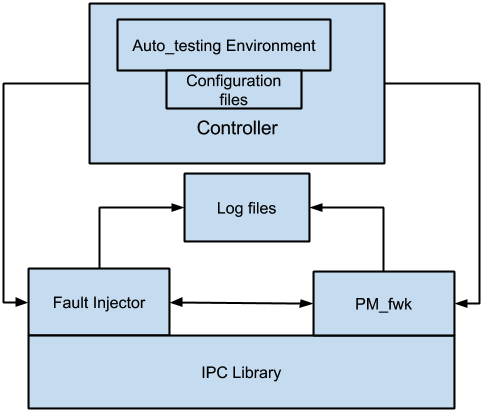
\includegraphics[width=\columnwidth]{figure/Fualt_injection_Model.png}
%\caption{Fault Injection Model \label{Fualt_injection_Model}}
%\end{figure}

\subsection{Challenges in adopting the fault injection approach}\label{sec:challenges}
During this study, we have met some challenges and barriers when adopting the fault injection approach. 
%Challenges started from understanding the existing system, since the software at the RBS in Ericsson is huge and complex as well as the number of the connected components are relatively high. 
%Furthermore, the idea of the fault injection is just available for cloud based application, but not to the embedded distributed system. So this study presents a new approach of fault injection that can be applicable to the embedded distributed system.  
%
%Another challenge was when we implemented the fault types, we implemented them from the scratch as well as imported some shared libraries in order to call some existing functionalities from the lower level. We met some difficulties in loading the IPC libraries as well as setting up the environment variables. After the implementation of the fault types, integrating the fault injection tool with the automatic testing environments was not a trivial task due to the strict conditions on the automatic testing environments. 
%
%There are some consideration that should be kept in mind when adopting this approach: 
%\begin{itemize}
%\item {\em Negative side effects}: When sending a lot of random messages without any time interval between the messages, 
% the system will probably crash since the computation power is limited on the embedded components. As stated in~\cite{Ali2014} online testing 
%could produce negative side effects out of the tester's control.
%It is then important to take into account also policies that help preventing or ameliorating such adverse
%effects. Also, as stated in~\cite{Ali2014}, online testing could have negative impact on nonfunctional characteristics; this can be mitigated by trading off
%testing accuracy with performance.
%%\item {\em Unrealistic results}: The testing method used in the fault injection approach is non-deterministic provocation thus the testing can catch unexpected faults that are seldom happened. When utilizing fault injection approach the results of the provoking can be both realistic and not realistic and this can be due to the fact that the input of the test is totally randomized. In order to mitigate from this limitation we made our test cases less randomized such as having time interval, specify the messages type, number of messages and delaying time. By doing this the result of the fault injection tool was more reasonable and at the same time it gave a realistic indicate when evaluating the system.
%\end{itemize} 

\noindent {\bf Unrealistic results}: Considering %Under the fact 
that %fault injection technique is 
we proposed a non-deterministic testing approach %that follow a randomized manner, 
the result of running such technique can be misleading. Doing a complete randomization of the test cases might produce useless results since the generating test case can be unrealistic. In order to mitigate this limitation we made our test cases less randomized such as having time interval, specify the messages type, number of messages and delaying time. 
For instance, when we implemented the first fault type, which was sending random messages, the system acts always differently. That was due to the fact that the injection is performed on embedded distributed systems with limited computation power. 
%where the computation power is limited, s
Sending a lot of random messages without any time between them was misleading. We come over this problem by inserting delays between each message sending. As a conclusion, having the time between each sending gave us a reasonable and realistic indication. 

\noindent {\bf Negative side effects}: When sending a lot of random messages without any time interval between them, 
 the system will probably crash since the computation power is limited on the embedded components. As stated in~\cite{Ali2014} online testing 
could produce negative side effects out of the tester's control.
It is then important to take into account also policies that help preventing or ameliorating such adverse
effects. Also, as stated in~\cite{Ali2014}, online testing could have negative impact on nonfunctional characteristics; this can be mitigated by trading off
testing accuracy with performance.

The strategy we adopted to avoid undesired crashes of the overall system because of injected fault is as follows:  
(i) Delaying signals - we make sure the delays fall within what the system should handle; (ii) Fuzzying signals - we limit fuzzying to faking Confirm/Rejects which the system should discard. %In the current state it is still hard for the PMFWK middleware to detect invalid Requests so that's left out.

%When we implemented the second fault type which was message delay, the system usually did not act as it should be, this was due to the fact that the time interval of delaying the messages was completely randomized. We come over this challenge by making it less randomized through identifying the default time and specifying the time interval. After that, the results were realistic and also gave us a reasonable indicate of approach evaluation. 
%Finally, continuous testing of the new implemented fault injection tool was time consuming. There are some steps that should be performed such as running the simulation and restarting the Erlang nodes in order to get and observe the result of testing in the log files. 



%Concluding, randomized fault injection can be an important test signal.

%\subsection{Altro}
%
%Online testing, however, poses two major challenges.
%First, it could produce negative side effects, out of the
%tester?s control, on the services of participating organizations.9
% The governance framework would thus need to
%include policies that help prevent or ameliorate such adverse
%effects, or compensate participating organizations
%in the event of serious consequences. Second, online testing
%could adversely impact nonfunctional characteristics.
%System engineers could mitigate this impact by trading off
%testing accuracy with performance.Preso da~\cite{Ali2014}




%\input{framework.tex}
%\input{instantiation.tex}
%\input{validation.tex}
%\input{discussion.tex}
\section{ Conclusion}\label{sec:conclusion}

This paper proposes a new fault injection approach to test distributed and embedded system with limited computation power. We performed the study in collaboration with Ericsson AB in Gothenburg, Sweden.
%study aimed to verify the robustness of the distributed system at Ericsson. 
%In particular, traditional testing techniques are used at Ericsson. However, t
%Traditional testing lacks of detecting the unexpected faults and dependency issues. We come over this problem by developing a new fault injection approach that performed based on non deterministic testing. Furthermore, t
This approach came as a complementary to traditional testing. As described in the paper, we developed the fault injection approach and the approach detected some unexpected faults. We observed also that fault injection can be adopted to test embedded distributed system and dependency bottlenecks can be identified. This approach provided the development team at Ericsson with 
%to utilize 
a better validation technique that permits to reduce the number of %and reduced from the 
unpredicted faults that appeared during the operations on the customers sides. %In the long run, using fault injection increases code quality, confidence level as well as reduces the cost.  %Academically, this thesis gave attention on the benefits of adopting such approach for fault tolerance ability of embedded distributed systems. In industry, generalizing this approach can help different companies that have a common interest in verifying the robustness of their embedded distributed system. 

As future work we plan to replicate the study to other organizations within Ericsson and to other companies  to better validate the generality of the approach. %make the approach more general.
%\subsection{Future work}
%This section shows some key improvements that can be considered for future work. This study focused on Ericsson environment. It would be interesting to involve more companies in the study for making more general approach to embedded distributed system, at the same time the result will be more reliable and general. In order to expand this approach and make it more general, the following suggestions can be taken into the consideration. 
We plan also to investigate steps that will permit to deploy the approach on customer production networks.  
%We plan also to integrate the approach with another testing technique such as mutation testing. Combining fault injection with mutation testing can be very effective and efficient, since fault injection tests the dependencies between the components and mutation testing tests the functionality of the system.  
%Previous research has described the strength of combining the fault injection with mutation testing in model based development~\cite{combinationtesting}. 

Finally, additional fault types can be injected such as register and memory faults, killing process, CPU overloads,  slow down network, fork bomb at a particular node, and drop network packets for duration of period at a certain rate, etc. %By injecting more fault types, the confidence level will be increased at the same time the total quality of the system will also be increased.  
It would also be an area of interest to test a combination of faults. This can be done by injecting a combination of faults in different order and at different time. %In this case the probability of detecting faults will increase for the reason of a larger set of input are involved in testing. 


%\begin{itemize}
%  \item Integrating this approach with another testing technique such as mutation testing.
%  \item Injecting the system with more fault types.
%  \item Make the same study on other companies and compare the result to see if it can be generic.
%  \end{itemize}

%\subsubsection{Integrating fault injection approach with mutation testing}
%
%Fault injection technique can be used in order to detect dependencies faults at the late stage of the development process. Utilizing fault injection approaches in an early stage is not the best practice. Therefore, combining fault injection techniques with mutation testing will improve the efficiency of detecting the faults at an early stage, thus reducing the cost as well as the time spend in detecting faults. Previous research has described the strength of combining the fault injection with mutation testing in model based development \cite{combinationtesting}.  
%
%Combining fault injection with mutation testing can be very effective and efficient, since fault injection tests the dependencies between the components and mutation testing tests the functionality of the system. Thus combining them will increase the confidence level of the internal and external code of the components as well as the consistencies between them. Moreover, the combined approach can be applied in an early stage and late stage of the development cycle. By doing this, the code will be validated continuously, the certainty level will be increased and bugs will be fixed in an early stage with lower cost.     

%\subsubsection{Injecting the system with more fault types}
%
%
%Due to time constrains we just focused on the two most potential fault types which are sending random messages as well as messages delaying. However, more fault types can be injected such as register and memory faults, killing process, CPU overloads,  slow down network, fork bomb at a particular node, and drop network packets for duration of period at a certain rate, etc. By injecting more fault types, the confidence level will be increased at the same time the total quality of the system will also be increased.  
%
%It would also be an area of interest to test a combination of faults. This can be by injecting a combination of faults in different order and at different time. In this case the probability of detecting faults will increase for the reason of a larger set of input are involved in testing. Furthermore, faults can act differently when injecting them in different order and different time \cite{FaaS}. Testing a combination of faults in a random based can detect even more unexpected faults. Moreover, this will increase the subset of the test suite that could be covered.    
%
%While fault injection is non deterministic testing that based on random manner, random testing can scale much more than deterministic testing \cite{random}. Particularly, the Ericsson system scales fast and using random testing will be cost effective in the long run. In this case the maintainability cost will not be at risk in case of updating the test suite.





			

\balance

\bibliographystyle{IEEEtran}
\bibliography{bibliography}

\end{document}